\documentclass[a4paper,11pt]{article}
\usepackage[T1]{fontenc}
\usepackage[utf8]{inputenc}
\usepackage{lmodern}
\usepackage{graphicx}
\usepackage[ngerman]{babel}


\title{model for data centric sensor faults}
\author{Maik Riestock}

\begin{document}

\maketitle
\tableofcontents

\begin{abstract}
This document presents a generic model for the description of data centric sensor faults. Based on this description is ..
\end{abstract}


\section{Concept}
 
 \begin{figure}[ht]
 	\centering
   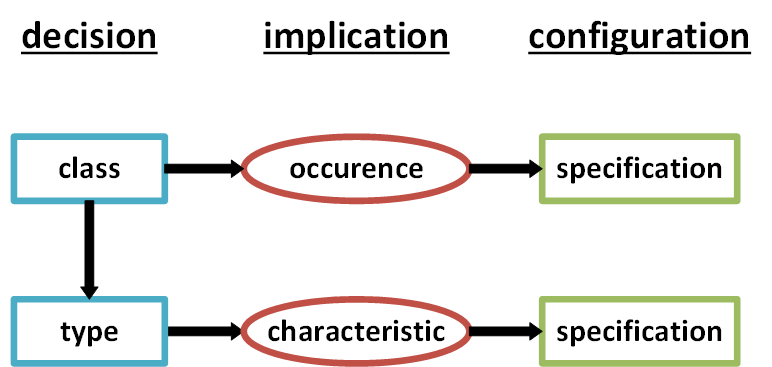
\includegraphics[width=0.7\textwidth]{graphics/Zeichnung2.png}
 	\caption{dont know yet}
 	\label{fig:concept}
 \end{figure}
 
\subsection{classes and types}  

define \textbf{classes}

Offset:..

Outlier:..


define \textbf{types}

non correlated:..

value correlated:..

time correlated:..



\subsection{occurence}

\begin{table}[h]
    \begin{center}
        \begin{tabular}{l||l}
		Type 							& Description	\\
		\hline
		permanent			& text..	\\
		transient				& text..	\\
		intermittent				& text..	\\

	\\													
        \end{tabular}
        \caption{Description of the various occurence modes}
        \label{tab:typen}
    \end{center}
\end{table}

\subsection{characteristic}

\begin{table}[h]
    \begin{center}
        \begin{tabular}{l||l}
		Type 							& Description	\\
		\hline
		non correlated				& text..	\\
		time correlated				& text..	\\
		value correlated				& text..	\\

	\\													
        \end{tabular}
        \caption{Description of the various characteristic modes}
        \label{tab:typen}
    \end{center}
\end{table}

\section{Implementation}

\subsection{modularisation}







\end{document}
